A major goal of robotics is to develop mobile robots that can operate fully autonomously in real world situations \cite{murphy2000introduction}.
These autonomous robots can be used for a wide range of applications.
For example, cleaning, inspection, transportation tasks or medical and construction assistance.
Robots can also operate in dangerous environments (e.g., life rescue or pollution control) without risking human lives.
Although much progress has been made, a truly autonomous robot that can operate in the real world, has not been developed yet.

One of the main prerequisites of an autonomous robot is the ability to known its position and movement in the environment.
Since no assumptions can be made about the environment, the robot has to learn from its environment.
This ability has been identified as a fundamental problem in robotics.
The process of incremental map construction and using it for localization is called \textbf{Simultaneous Localization and Mapping (SLAM)}.
Its main function is to aggregate observations obtained by sensors in order to obtain information of the environment and store it in a map.
This location information is used by other subsystems of the robot, such as interaction with the environment.
%depending on the robot's task.
%This process was inspired by the the human ability to learn maps of the surrounding environment and to use them for localization.

A wide range of SLAM methods have been presented.
These methods include various sensor configurations to obtain map information as well as knowledge about the robots location.
%A wide range of methods have been presented, depending on the application environment and the a-priori information about it.
Available solutions for certain environments and sensor configurations are well understood.
For other environments and sensor configurations, open problems remain.
%These are issues regarding map representation and its uncertainty, real-time capable update methods and sensor fusion %algorithms. Almost every technique assumes the environment to be static.
%A more difficult problem occurs if the environment changes over time.
One of them is SLAM with micro aerial vehicles (MAVs), which have a limited sensor suite due to their weight constraints.

\begin{figure}[htb]
\centering
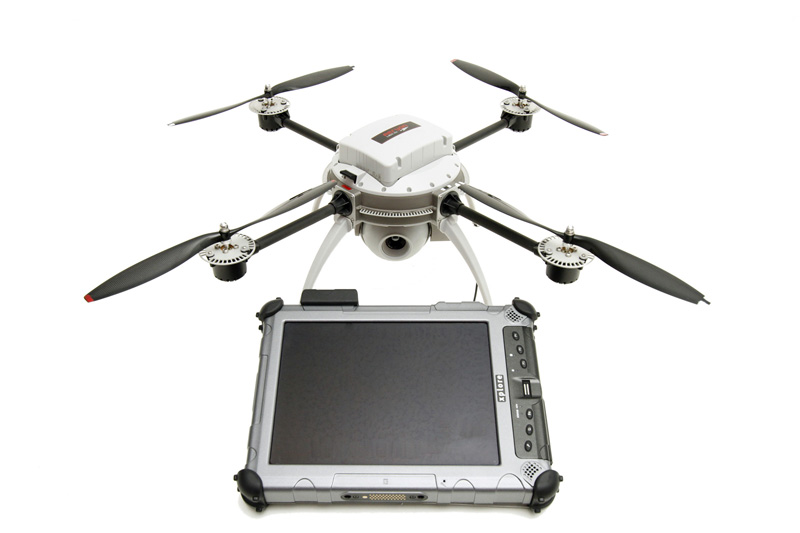
\includegraphics[width=11.0cm]{images/aeryon-scout-tablet.jpg}
\caption{The Aeryon Scout is an unmanned micro aerial vehicle, used for tactical, over-the-hill aerial intelligence. The platform is controlled by a touchscreen interface and is able to fly pre-planned flight paths using GPS positioning.}
\label{fig:introduction_aeryon_scout}
\end{figure}

A \textbf{micro aerial vehicle (MAV)} is a class of unmanned aerial vehicles (UAV).
Their small size allows a wide range of robotic applications, such as surveillance, inspection and search \& rescue.
An example of a MAV developed for surveillance and inspection is the Aeryon Scout\footnote{\url{http://www.aeryon.com/products/avs.html}} (Figure \ref{fig:introduction_aeryon_scout}), which is already being deployed in the field\footnote{\url{http://www.aeryon.com/news/pressreleases/271-libyanrebels.html}}.
Particularly interesting are small quadrotor helicopters, which are lifted and propelled by four rotors.
They offer great maneuverability and stability, making them ideal for indoor and urban flights.
Due to technical developments in the last years, small quadrotors with on-board stabilization like the Parrot AR.Drone can be bought off-the-shelf.
These quadrotors make it possible to shift the research from basic control of the platform towards intelligent applications that require information about the surrounding environment.
However, the limited sensor suite and the fast movements make it quite a challenge to use SLAM methods for such platforms.

%	\section{Versatile scouting capabilities of a quadrotor helicopter}


	\section{International Micro Air Vehicle competition}
\label{sec:introduction-imav}
The International Micro Air Vehicle competition (IMAV) is an effort to stimulate the practical demonstration of MAV technologies.
The competitions have as goal to shorten the road from novel scientific insights to application of the technology in the field.
Since the Summer 2011 edition of IMAV, teams can borrow a Parrot AR.Drone quadrotor helicopter.
This allows teams to focus research on the artificial intelligence part of the competitions.

Currently, IMAV has three distinct competitions: two indoor competitions and one outdoor competition.
One of the indoor competitions is the Pylon challenge (Figure \ref{fig:imav2011_pylon}).
The objective of the Pylon challenge is to navigate a MAV in figure-8 shapes around two poles.
The competition rules\footnote{\url{http://www.imav2011.org/images/stories/documents/imav2011-summerediton_indoor_challenges_v3.0.pdf}} have been created to stimulate the level of autonomy; significantly more points are given to fully autonomous flights.

\begin{figure}[htb]
\centering
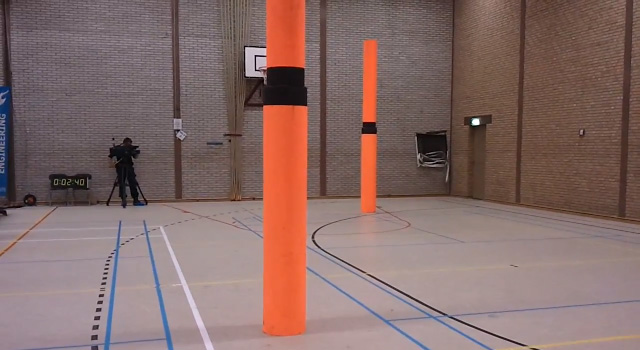
\includegraphics[width=11cm]{images/imav2011_pylon.jpg}
\caption{The IMAV2011 Pylon challenge environment, which is located in a sports gym.
The objective is to navigate a MAV in figure-8 shapes around two poles that are $10\small{m}$ apart. Each pole has a height of approximately $4\small{m}$.}
\label{fig:imav2011_pylon}
\end{figure}

The main bottleneck for indoor autonomy is reliable indoor positioning.
Team are allowed to use external aids to solve their positioning problem, at the cost of points.
Examples of external aids are visual references (markers) and radio positioning beacons.
One of the contributions of this thesis is the development of basic navigation capabilities for the AR.Drone, without relying on external aids.
These navigation capabilities can be used during the IMAV competitions, allowing fully autonomous flights.
%This thesis is an effort to develop 
%These navigation capabilities can be used during the IMAV competitions, allowing fully autonomous flights.

	\section{RoboCup Rescue}
Another effort to promote research and development in robotics is RoboCup \cite{kitano1997robocup}.
The RoboCup competions have as goal to stimulate research by providing standard problems where wide range of technologies can be integrated and examined.
Unlike the IMAV competitions, the RoboCup competitions are not limited to MAVs.

The RoboCup Rescue league \cite{kitano1999robocup} is part of the RoboCup competitions.
This league aims at the development of robotic technology that could 
%effectively
help human rescuers in the aftermath of disasters like earthquakes, terroristic attacks and other extreme situations.
In addition to a Rescue league with real robots, the Virtual Robots Competition was started, which uses a simulator instead of real robots.
Simulation has some \mbox{significant} advantages above real competitions, such as the low costs and the ability to easily construct different disaster scenarios.

The main bottleneck for robot simulation is the requirement of realistic motion and sensor models.
The simulation environment selected for the Virtual Robots Competition is USARSim \cite{Balakirsky2009iros,carpin2007usarsim}, which includes models of a wide range of robotic platforms and sensors.
Unfortunately, the support of aerial vehicles in USARSim is little, while MAVs offer great advantages above other robots due to the versatile scouting capabilities.
In 2011, the expensive AirRobot quadrotor was the only aerial vehicle available in USARSim.
One of the contributions arising from this thesis is a simulation model of the affordable AR.Drone quadrotor.
The resulting model can be used by teams to make use of the advantages of MAVs in disaster scenarios.


	\section{Objectives and research questions}
One goal of robotics is to develop mobile robots that can operate robustly and fully autonomously in real world situations \cite{murphy2000introduction}.
One of the main prerequisites of an autonomous robot is the ability to know its location and movement in the environment \cite{talluri1992position}.
Since no assumptions can be made about the environment, the robot has to learn from its environment.

Simultaneous Localization and Mapping using aerial vehicles is an active research area in robotics.
However, current approaches use algorithms that are computationally expensive and cannot be applied for real-time navigation problems.
Furthermore, other researchers rely on expensive aerial vehicles
%equipped
with advanced sensors like a laser rangefinder.
Focusing on real-time methods and affordable MAVs increases the employability of aerial vehicles in real world situations.
In case of semi-autonomous robots, building and visualizing an elevated and textured map of the environment offers additional feedback to the teleoperator of the vehicle.

The main research question therefore is to determine a real-time Simultaneous Localization and Mapping approach that can be used for MAVs with a low-resolution down-pointing camera (e.g., AR.Drone).
This main research question is divided into several sub-questions:
\begin{itemize}
\item How to construct a texture map and a feature map from camera frames?
%\item What camera resolution (e.g., $176 \times 144$ pixels) is required for localization against a map? What is the relationship between camera resolution and the localization performance?
\item What is the relation between camera resolution and localization performance? Is a camera resolution of $176 \times 144$ pixels enough to localize against a map?
\item What is the performance and robustness of different methods to estimate the transformation between a camera frame and a map?
\item Is localization on regular basis possible for circumstances encountered during the IMAV competition?
\item How to construct an elevation map with a single ultrasound sensor?
%\item What is the quality of the produced visual maps [in terms of human navigation purposes]?
%\item How useful are the produced visual maps for human navigation purposes?
\end{itemize}

In order to perform (global) localization, a map of the environment has to be constructed.
Considering the limited sensor suite of affordable quadrotors (e.g., AR.Drone), camera images are often the best information source for localization and mapping.
This poses the questions how to construct a map from camera frames.
The AR.Drone is equipped with a very low-resolution camera, which poses the question if localization against a map is possible with such cameras.
The recent developments in miniaturizing high-resolution cameras enables MAVs to be equipped with high-resolution cameras.
This leads to the question how the (increasing) image resolution will affect the localization performance.
When a map is constructed, the camera frames are matched against the map to perform (global) localization.
A robust transformation is computed to describe the relation between the vehicle's position and the map.
Different transformation estimation methods can be used and have to be compared.
The performance of the localization method is also depending on the environment.
Circumstances encountered during the IMAV competition are challenging due to the repeating patterns (lines) and the lack of natural features.
Therefore, the localization method is evaluated for such circumstances.
Finally, an elevation map is constructed using a single airborne ultrasound sensor.
Since no method has been proposed by others, the question arises how to construct this map.





\section{Contributions}
The first contribution of this thesis is a framework that aids in the development of (intelligent) applications for the AR.Drone.
The framework contains an abstraction layer to abstract from the actual device, which allows to use a simulated AR.Drone in a way similar to the real AR.Drone.
Therefore, a simulation model of the AR.Drone is developed in USARSim.
The main contribution is a new approach that enables a MAV with a low-resolution down-looking camera to navigate in circumstances encountered during the IMAV competition.
An algorithm is presented to robustly estimate the transformation between a camera frame and a map.
In addition to the navigation capabilities, the approach generates a texture map, which can be used for human navigation.
Another contribution is a method to construct an elevation map with an airborne ultrasound sensor.

	\section{Outline}
\textbf{Chapter \ref{chapter:probabilistic-robotics} and \ref{chapter:computer-vision}} give an overview of the background theory that is part of the presented methods.
This theory includes probabilistic robotics (Chapter \ref{chapter:probabilistic-robotics}) and computer vision techniques (Chapter \ref{chapter:computer-vision}).
In \textbf{Chapter \ref{chapter:related-research}}, an overview of related research is given.
This research is divided into three segments: SLAM methods for building texture maps, elevation mapping with ultrasound sensors and research conducted with the AR.Drone.
An extensive overview of the AR.Drone platform is presented in \textbf{Chapter \ref{chapter:platform}}.
The platform overview covers the hardware, the quadrotor flight control and finally its Application Programming Interface (API).
This API lacks functionalities to employ a SLAM method.
Therefore, it is extended to a development framework in \textbf{Chapter \ref{chapter:development-environment}}.
In addition to this framework, a realistic simulation model of the AR.Drone is developed.
This simulation model allows safe and efficient development and testing of algorithms.
\textbf{Chapter \ref{chapter:visual-slam}} presents the Visual SLAM method for the AR.Drone.
It includes pose estimation, real-time mapping, localization using the map and building an elevation map using a single ultrasound sensor.
\textbf{Chapter \ref{chapter:results}} describes the conducted experiments and presents the results.
In \textbf{Chapter \ref{chapter:conclusions}}, this thesis concludes by answering the research questions and summarizing directions for future research.